\begin{frame}{There is \st{an App} a Package for that!}

\begin{center}
{\fontsize{100}{90}\selectfont 68829!}
\end{center}
\vfill

\textcolor{gray}{\tiny (2016-12-01) \\ wget http://packages.ubuntu.com/xenial/allpackages?format=txt.gz -q -O - | zcat | tail -n +6 | wc -l}
\end{frame}


\begin{frame}{Achtung}
\begin{center}
\texttt{@draget} $ \rightarrow $ 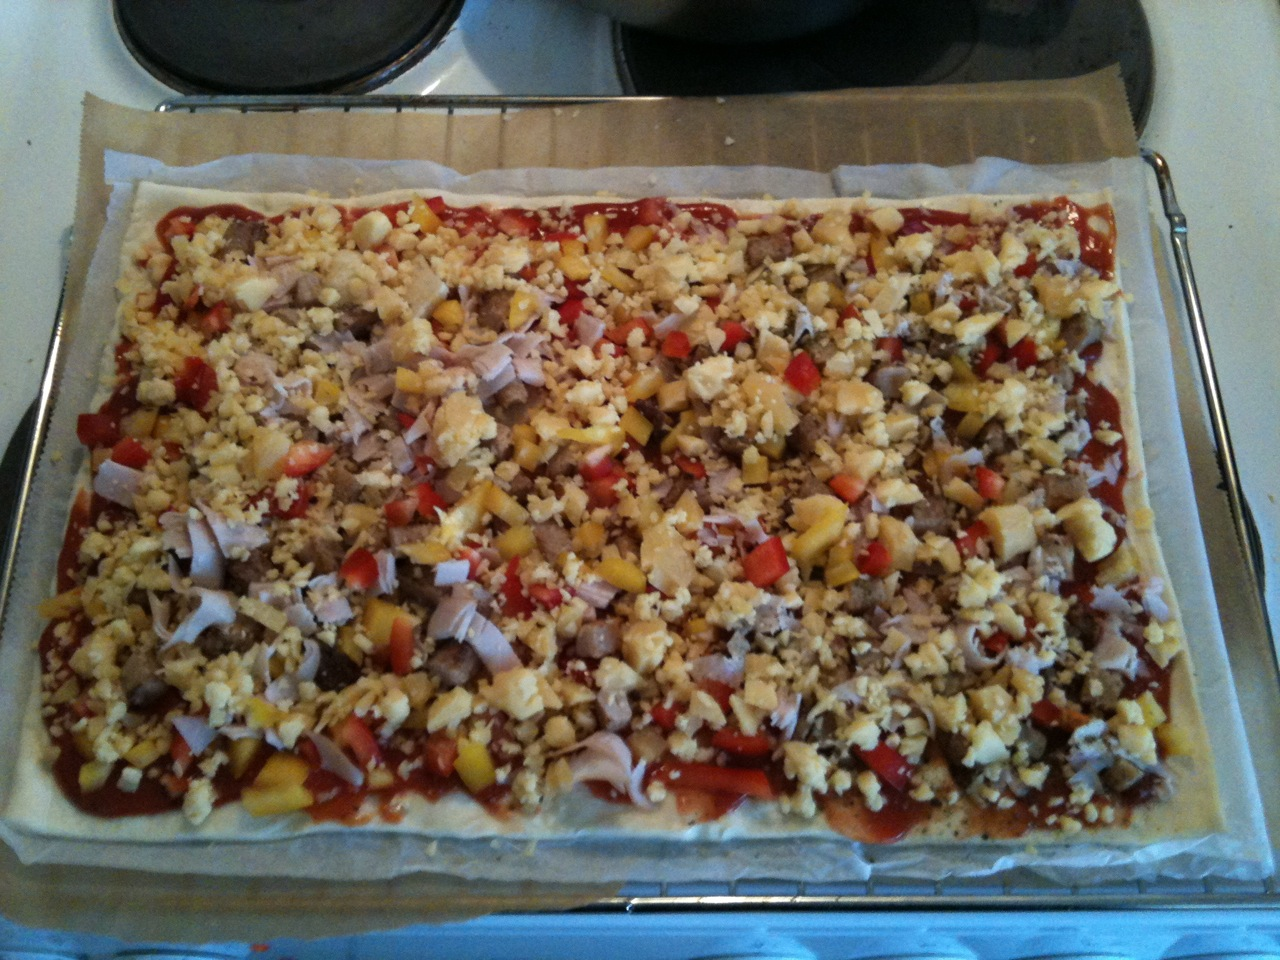
\includegraphics[scale=0.12]{images/draget}
\end{center}
\begin{itemize}
\item Die hier vorgestellte Software ist eine persönliche Auswahl des Vortragenden
\item Vorschläge oder Fragen gewünscht!
\end{itemize}
\end{frame}

\begin{frame}{GPL, Fuck Yeah!}
Fast jede hier vorgestellte Software ist:
\begin{itemize}
\item kostenlos!
\item quelloffen!
\item aus Spaß am Entwickeln entstanden!
\end{itemize}
\end{frame}